\documentclass{article}
\usepackage{graphicx}
\usepackage{float}
\usepackage{amsmath,amsthm,amssymb}

\title{MLCD Homework 3}
\date{December 5th 2013}
\author{David Snyder, dsnyde29
        \and Adi, adi ID}

\usepackage{amsmath,amsthm,amssymb}

\begin{document}
\maketitle

\section*{Variation Inference on a Simple Network}
\subsection*{2.1.a}

\begin{proof}
   Assume the posterior is factored according to the mean-field distribution:
   $q(\textbf{x}) = \prod_{i=1}^{D} q_{i}(\textbf{x}_{i})$ 
   where $x \in \{A,B,C,D,E,F\}$.
   We need to find the $q$ such that $\mathcal{K}\mathcal{L} (q \mid \mid p)$ is minimized.
   From equation 21.9 of Murphy we have that this is equivalent to minimizing the lower
   bound on the energy functional $J(q) \ge -log(p(D))$ or equivalently, maximixing the
   lower bound: $L(q) = log(p(D))$.
  \begin{align*}
     L(q_{j}) &= \sum_{x} \prod_{i} q_{i} (\textbf{x}_{i}) (log(\hat{p} (\textbf{x})) - \sum_{k} log(q_{k} (\textbf{x}_{k}))) \\
     &= \sum_{x_{j}} \sum_{x_{-j}} q_{j} (\textbf{x}_{j}) \prod_{i \ne j} q_{i}(\textbf{x}_{i}) (log(\hat{p}(\textbf{x})) - \sum_{k} log(q_{k}(\textbf{x}_{k}))) \\
     &= \sum_{x_{j}} q_{j}(\textbf{x}_{j} \sum_{\textbf{x}_{-j}})) \prod_{i \ne j} q_{i}(\textbf{x}_{j})(\sum_{k \ne j} log(q_{k}(\textbf{x}_{k}) + q_{j}(\textbf{x}_{j})) \\
     &= \sum_{x_{j}} q_{j}(\textbf{x}_{j}) log(f_{j}(\textbf{x}_{j}) - \sum_{x_{j}} q_{j}(\textbf{x}_{j} log(q_{j}(\textbf{x}_{j})) + C \\
 \end{align*}
 Where $f_{j}(\textbf{x}_{j}) \propto exp(\sum_{\textbf{x}_{-j}} \prod_{i \ne j } q_{i}(\textbf{x}_{i}) log( \hat{p}(\textbf{x})))$.
This allows us to write $L(q_{j}) = - \mathcal{K} \mathcal{L} (q_{j} \mid \mid f_{i})$ once we drop terms which are constant with respect to $q_{j}$. We can minimize this by setting $q_{j} = f_{j}$,
 giving us $q_{j}(\textbf{x}_{j}) \propto exp(\sum_{\textbf{x}_{-j}} \prod_{i \ne j } q_{i}(\textbf{x}_{i}) log( \hat{p}(\textbf{x})))$.
 We only need to consider nodes in $\textbf{x}_{j}$'s Markov blanket (21.3 Murphy), so we don't need to multiply over all $q(\textbf{x}_{i})$.
\end{proof}
We can now write the final form of the update equations:
\begin{itemize}
  \item $q_{A}(a) \propto exp(\sum_{b,c} q_{B}(b) q_{C}(c) log( p(a)p(b \mid a)p(c \mid a,b)))$
  \item $q_{B}(b) \propto exp(\sum_{a,c,d} q_{A}(a) q_{C}(c) q_{D}(d) log(p(d \mid b,d) p(d \mid b) p(c \mid a,b)))$
  \item $q_{C}(c) \propto exp(\sum_{a,b,d,e} q_{A}(a) q_{B}(b) q_{C}(c) q_{D}(d) q_{E}(e) log(p(c \mid a,b) p(e \mid c,d)$
  \item $q_{D}(d) \propto exp(\sum_{b,c,e,f} q_{B}(b) q_{C}(c) q_{E}(e) q_{F}(f) log(p(d \mid b,d) p(f \mid f,d) p(e \mid c,d)$
  \item $q_{E}(e) \propto exp(\sum_{c,d,f} q_{C}(c) q_{D}(d) q_{F}(f) log(p(e \mid c,d)$
  \item $q_{F}(f) \propto exp(\sum_{d,e} q_{D}(d) q_{E}(e) log(p(f \mid d)$
\end{itemize}


\subsection*{2.1.b}
See inference.R for an implementation of the mean-field update equations.

Using the mean-field approximation, we get a KL divergence of about .83 for computing the marginal over $E$ and $F$. The measurement corresponds to a sort of distance, telling us how much information we've lost by approximating $p(E,F)$ by $q(E)q(F)$. This estimate is probably not very reasonable, since it assumes that there is little to no dependence between each variable, although the CPTs shows that there is.

\subsection*{2.1.c}
Note: we handle this derivation in a similar way to mean-field. Because of this, the derivation only holds for non-overlapping structures, such as the $\{A,B,C\}$ and $\{D,E,F\}$.

\begin{proof}
   Assume the posterior is factored according to the mean-field distribution:
   $q(\textbf{c}) = \prod_{i=1}^{D} q_{i}(\textbf{c}_{i})$ 
   where cluster $c \in \{\{A,B,C\},\{D,E,F\}\}$.
   We need to find the $q$ such that $\mathcal{K}\mathcal{L} (q \mid \mid p)$ is minimized.
   From equation 21.9 of Murphy we have that this is equivalent to minimizing the lower
   bound on the energy functional $J(q) \ge -log(p(D))$ or equivalently, maximixing the
   lower bound: $L(q) = log(p(D))$.
  \begin{align*}
     L(q_{j}) &= \sum_{c} \prod_{i} q_{i} (\textbf{x}_{i}) (log(\hat{p} (\textbf{c})) - \sum_{k} log(q_{k} (\textbf{c}_{k}))) \\
     &= \sum_{c_{j}} \sum_{c_{-j}} q_{j} (\textbf{c}_{j}) \prod_{i \ne j} q_{i}(\textbf{c}_{i}) (log(\hat{p}(\textbf{c})) - \sum_{k} log(q_{k}(\textbf{c}_{k}))) \\
     &= \sum_{c_{j}} q_{j}(\textbf{c}_{j} \sum_{\textbf{c}_{-j}})) \prod_{i \ne j} q_{i}(\textbf{c}_{j})(\sum_{k \ne j} log(q_{k}(\textbf{c}_{k}) + q_{j}(\textbf{c}_{j})) \\
     &= \sum_{c_{j}} q_{j}(\textbf{c}_{j}) log(f_{j}(\textbf{c}_{j}) - \sum_{c_{j}} q_{j}(\textbf{c}_{j} log(q_{j}(\textbf{c}_{j})) + C \\
 \end{align*}
 Where $f_{j}(\textbf{c}_{j}) \propto exp(\sum_{\textbf{c}_{-j}} \prod_{i \ne j } q_{i}(\textbf{c}_{i}) log( \hat{p}(\textbf{c})))$.
This allows us to write $L(q_{j}) = - \mathcal{K} \mathcal{L} (q_{j} \mid \mid f_{i})$ once we drop terms which are constant with respect to $q_{j}$. We can minimize this by setting $q_{j} = f_{j}$,
 giving us $q_{j}(\textbf{c}_{j}) \propto exp(\sum_{\textbf{c}_{-j}} \prod_{i \ne j } q_{i}(\textbf{c}_{i}) log( \hat{p}(\textbf{c})))$.
 We only need to consider nodes in the Markov blanket of nodes in $\textbf{c}_{j}$ (21.3 Murphy), so we don't need to multiply over all $q(\textbf{c}_{i})$.
\end{proof}
We can now write the final form of the update equations:
\begin{itemize}
  \item $q_{A,B,C}(a,b,c) \propto exp(\sum_{d,e,f} q_{D}(d) q_{E}(e) q_{F}(f) log( p(a)p(b \mid a)p(c \mid a,b) p(d \mid b) p(e \mid c,d)))$
  \item $q_{D,E,F}(d,e,f) \propto exp(\sum_{b,c} q_{B}(b) q_{C}(c) log( p(f \mid d)p(e \mid c,d) p(d \mid b) ))$
\end{itemize}

\subsection*{2.1.d}
See inference.R for an implementation of the structured meanfield
update equations. This is indeed a better approximation than the mean-field. We get a KL divergence of about 0.002 instead of 0.83. This redunction in KL divergence corresponds to a lower amount of uncertainty by encoding $p(E,F)$ with $\sum_{d} q(d,E,F)$. There is a lot of 
dependence between the variables in the Bayesian network. This
is evident both in the $CPT$ as well as the lower KL divergence for
the structured mean-field. The fully factored mean-field would only
have been a good approximation if there was indeed very little
dependence between variables.

\section*{Collapsed Gibbs Sampler}
The collapsed gibbs sampler was implemented and a shell script to run the sampler is provided.
./collapsed-sampler "input train file" "input test file" "output file preffix" "number of topics" "lambda" "alpha" "beta" "iterations" "burn-in"

Using this we generated the following output files, using different values for K (5 and 25), lambda (0.5, 0.8, 0.2)
and alpha(0.1 and 1.0). 1100 iterations were completed with 1000 burn in iterations.\\
collapsed-output-25-0.2-0.1.txt-phi\\
collapsed-output-25-0.2-0.1.txt-phi0\\
collapsed-output-25-0.2-0.1.txt-phi1\\
collapsed-output-25-0.2-0.1.txt-testll\\
collapsed-output-25-0.2-0.1.txt-theta\\
collapsed-output-25-0.2-0.1.txt-trainll\\
collapsed-output-25-0.5-0.1.txt-phi\\
collapsed-output-25-0.5-0.1.txt-phi0\\
collapsed-output-25-0.5-0.1.txt-phi1\\
collapsed-output-25-0.5-0.1.txt-testll\\
collapsed-output-25-0.5-0.1.txt-theta\\
collapsed-output-25-0.5-0.1.txt-trainll\\
collapsed-output-25-0.5-1.txt-phi\\
collapsed-output-25-0.5-1.txt-phi0\\
collapsed-output-25-0.5-1.txt-phi1\\
collapsed-output-25-0.5-1.txt-testll\\
collapsed-output-25-0.5-1.txt-theta\\
collapsed-output-25-0.5-1.txt-trainll\\
collapsed-output-5-0.5-0.1.txt-phi\\
collapsed-output-5-0.5-0.1.txt-phi0\\
collapsed-output-5-0.5-0.1.txt-phi1\\
collapsed-output-5-0.5-0.1.txt-testll\\
collapsed-output-5-0.5-0.1.txt-theta\\
collapsed-output-5-0.5-0.1.txt-trainll\\
collapsed-output-5-0.8-0.1.txt-phi\\
collapsed-output-5-0.8-0.1.txt-phi0\\
collapsed-output-5-0.8-0.1.txt-phi1\\
collapsed-output-5-0.8-0.1.txt-testll\\
collapsed-output-5-0.8-0.1.txt-theta\\
collapsed-output-5-0.8-0.1.txt-trainll\\


\section*{5 Blocked Gibbs Sampler}
\subsection*{5.1 Derivation}

\section*{6 Text Analysis}
\subsection*{6.1}

\begin{figure}[H]
  \caption{Training and Test log likelihoods (chain 1)}
  \centering
    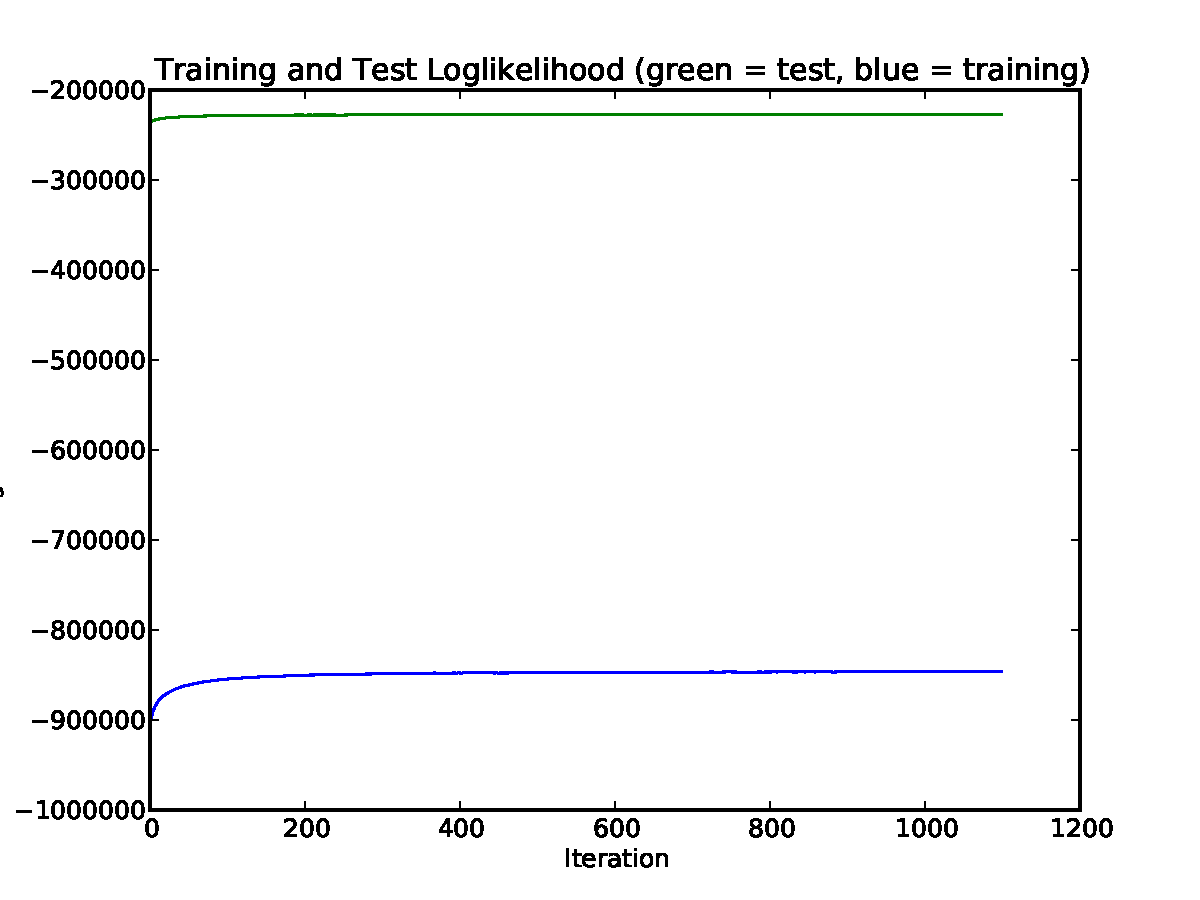
\includegraphics[width=1.0\textwidth]{q6_p1_1.pdf}
\end{figure}

\begin{figure}[H]
  \caption{Training and Test log likelihoods (chain 2)}
  \centering
    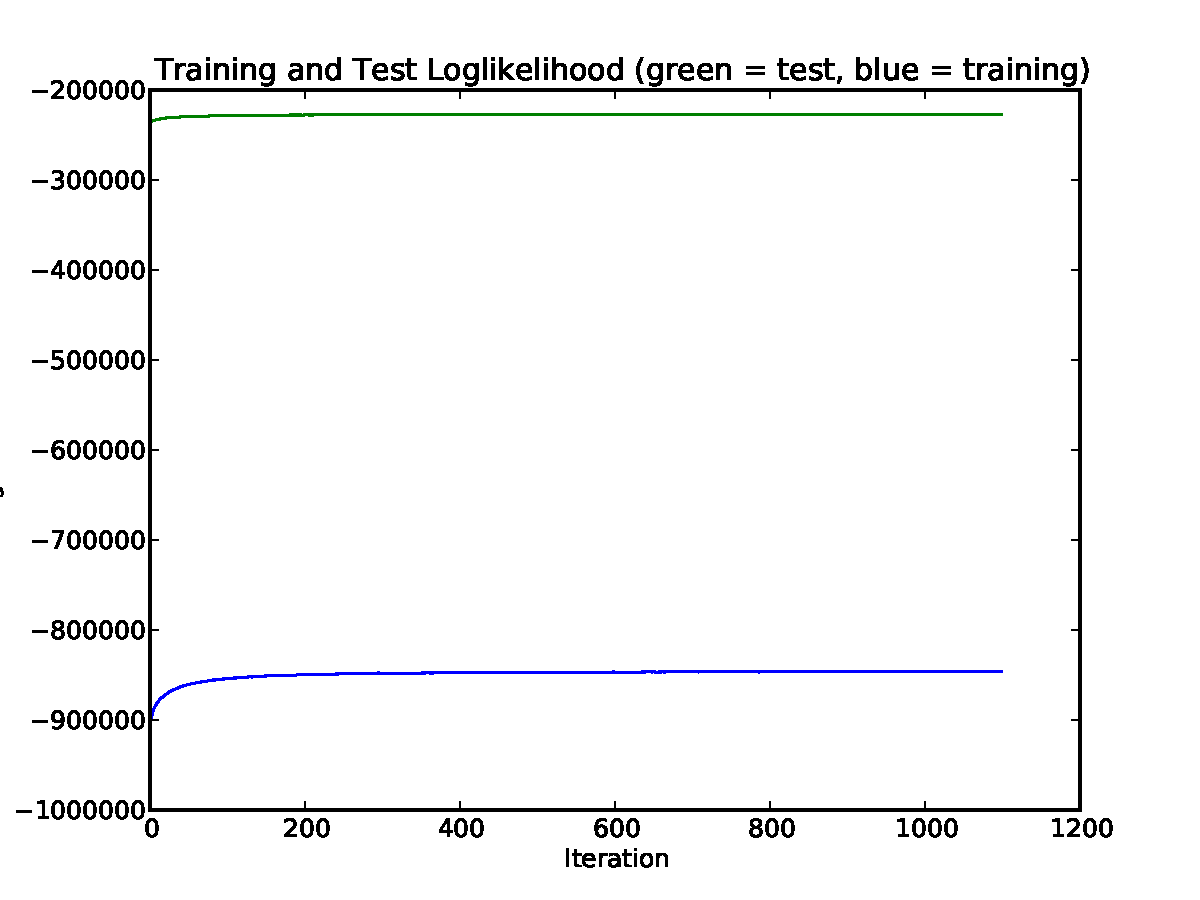
\includegraphics[width=1.0\textwidth]{q6_p1_2.pdf}
\end{figure}

\begin{figure}[H]
  \caption{Training and Test log likelihoods (chain 3)}
  \centering
    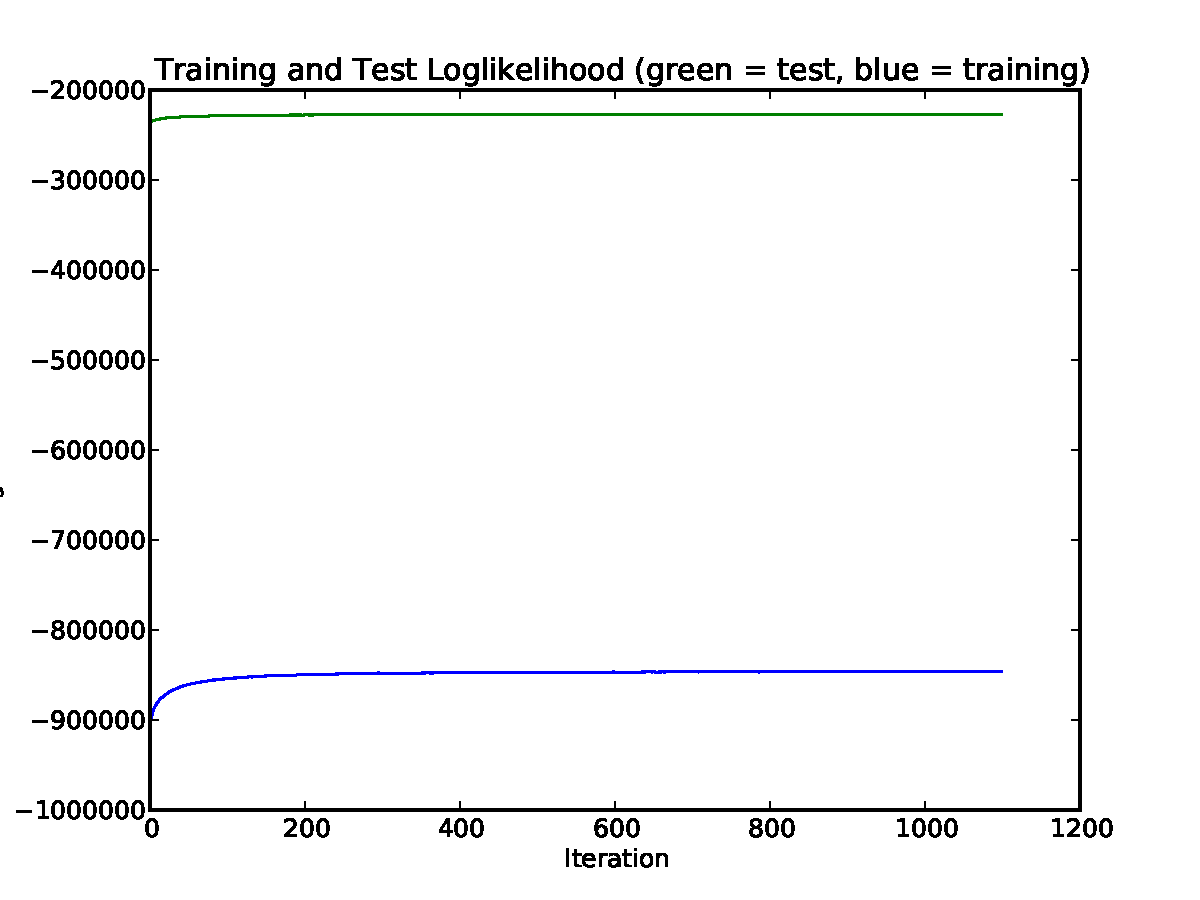
\includegraphics[width=1.0\textwidth]{q6_p1_2.pdf}
\end{figure}

We've plotted the test and training log likelihood as a function of
the number of iterations. Each plot exhibits the same trends; the training log likelihood increases over a period
of about 100 iterations, before leveling off, while the test log likelihood behaves asymptotically after about 50 iterations. The
log likelihood of the test data is much higher than that of the training log likelihood, because the test data is much smaller.

\subsection*{6.2}

Extra Credit

\subsection*{6.3}

Extra Credit

\subsection*{6.4}
\begin{figure}[H]
  \caption{Test log likelihood vs topic size}
  \centering
    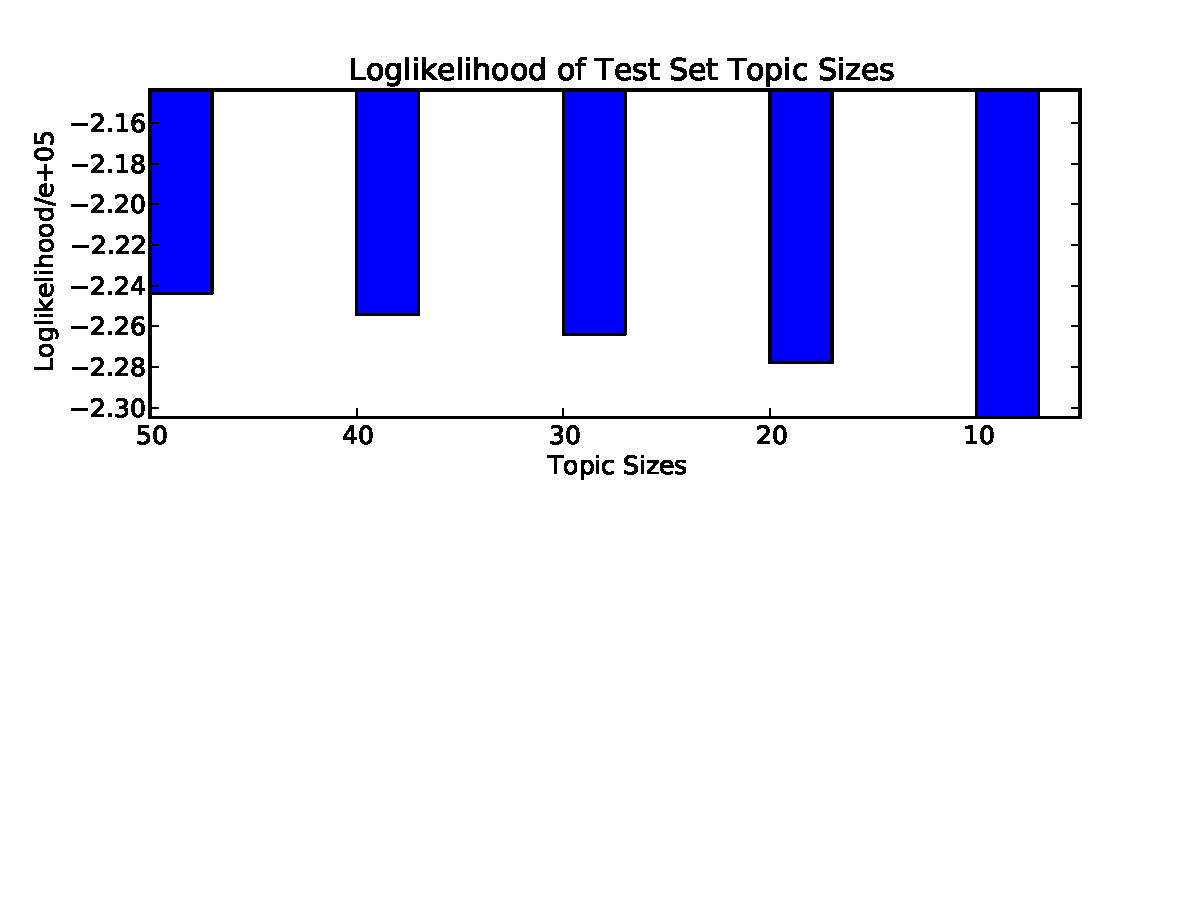
\includegraphics[width=1.0\textwidth]{q6_p4.pdf}
\end{figure}
The test likelihood increases with number of topics. The likelihood was highest for a topic size of 50.

\subsection*{6.5}
\begin{figure}[H]
  \caption{Test log likelihood as a function of lambda)}
  \centering
    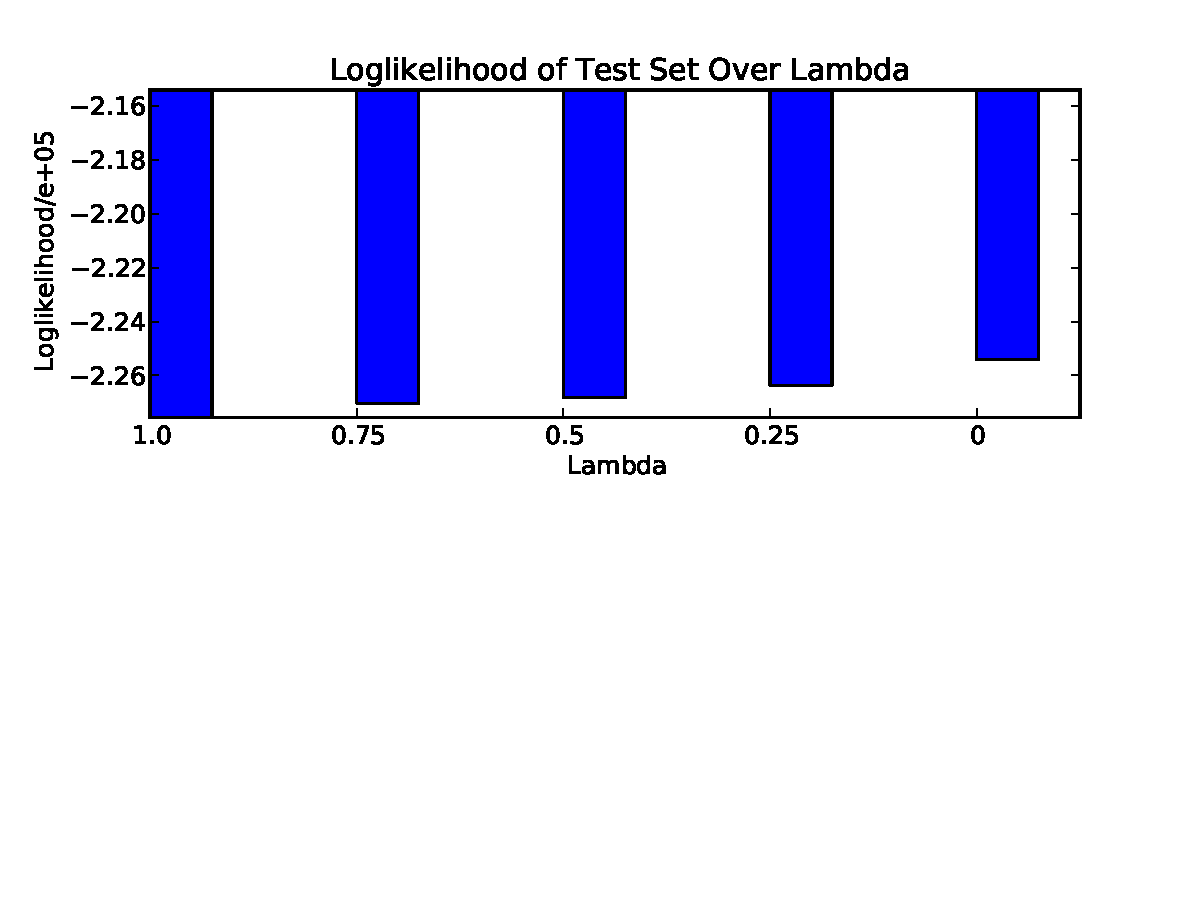
\includegraphics[width=1.0\textwidth]{q6_p5.pdf}
\end{figure}

We see that as lambda decreases the log likelihood
increases. For instance, at lambda = 1.0 the log likelihood is about -2.28e+05, while at lambda = 0 the log likelihood is about
-2.255e+05.

\subsection*{6.6.a}
Below is an example of topics from ACL, NIPS and global that share a common theme:\\
ACL\\
Topic 1\\
model 0.016177074286\\
models 0.0115966992618\\
algorithm 0.0111221444474\\
probability 0.0100090151025\\
statistical 0.00885346456302\\
parsing 0.00821317593643\\
problem 0.00780716347197\\
based 0.00749694584482\\
given 0.00747310208966\\
data 0.00742426483454\\
using 0.00720128594085\\
maximum 0.00711986474806\\
grammar 0.00653818196435\\
probabilities 0.00591095459551\\
approach 0.00582103926486\\
algorithms 0.00580315705065\\
tree 0.00551910860789\\
time 0.00540066553474\\
grammars 0.00533389632103\\
framework 0.00530399171093\\
NIPS\\
Topic 0\\
algorithm 0.0218752931149\\
model 0.0147504470285\\
data 0.0144234378009\\
models 0.0110908058826\\
linear 0.010814378643\\
method 0.00987114130807\\
function 0.00961977446919\\
learning 0.00949037931016\\
problem 0.0088664442374\\
using 0.00817617120279\\
analysis 0.00789862326851\\
results 0.00742700154592\\
approach 0.00740190068817\\
non 0.00720331878952\\
probability 0.00708074495813\\
new 0.0069104242882\\
present 0.00653868103357\\
algorithms 0.00651221863588\\
gaussian 0.00629224913294\\
based 0.00609463801093\\
Global\\
Topic 0\\
algorithm 0.0180317637371\\
model 0.0153512978987\\
data 0.0119218228652\\
models 0.0113371360174\\
problem 0.00852501154491\\
linear 0.00821802077018\\
probability 0.00819562127406\\
method 0.00814143246541\\
using 0.00786159924427\\
learning 0.00731179331377\\
function 0.00725015695961\\
approach 0.00685902616221\\
based 0.00664327777912\\
statistical 0.00647947181681\\
results 0.00641035322625\\
algorithms 0.00628478063586\\
new 0.00618878561834\\
analysis 0.00603455553512\\
non 0.00576769211681\\
present 0.00565615967426\\

These topic themes seems most similar even for different number of topics. (K=10,20,30)
Another topic that was similar across all three corpora was:
ACL:\\
Topic 13\\
learning 0.0236569277439\\
data 0.0193323907822\\
training 0.0177041124081\\
performance 0.0159465697687\\
number 0.0124777968224\\
classification 0.0124619741943\\
task 0.0116708930056\\
features 0.011406526229\\
method 0.00993581517459\\
machine 0.00986731144034\\
problem 0.00986126749427\\
based 0.00981922475935\\
results 0.00958337539838\\
set 0.00951327638253\\
methods 0.00951126987734\\
tasks 0.00915523901263\\
classifiers 0.00896529773783\\
supervised 0.00872972939337\\
small 0.0081479403109\\
paper 0.00804743671283\\
\\
NIPS:\\
Topic 13\\
data 0.0300396007649\\
learning 0.0297261962164\\
training 0.019597857133\\
method 0.0184479683093\\
classification 0.0171312523806\\
classifier 0.0145576037986\\
algorithms 0.0139714522147\\
performance 0.0133121610783\\
problem 0.0126331017797\\
set 0.0117619073234\\
class 0.0116415049338\\
methods 0.0116134797214\\
results 0.0116030737418\\
vector 0.011232450178\\
new 0.0111925377437\\
large 0.011071185214\\
based 0.0104201924844\\
number 0.0099513554648\\
paper 0.00978429669297\\
solution 0.00951159481878\\
\\
Global:\\
Topic 13\\
learning 0.026646969666\\
data 0.0243572607502\\
training 0.0187586479328\\
performance 0.0149455191817\\
classification 0.0147060786892\\
method 0.0138767816174\\
number 0.0114753712323\\
problem 0.0112215436682\\
classifier 0.0108612392988\\
algorithms 0.0107930679265\\
set 0.0106309255965\\
results 0.010596472879\\
methods 0.0105545761066\\
based 0.0102011322731\\
task 0.00961196420842\\
large 0.00940082405471\\
features 0.00933764214712\\
vector 0.0092084187336\\
tasks 0.0091929993896\\
paper 0.00892055841457\\

We found some instances of where the global would match one of the corpus, but none where all three matched strongly.

When looking for different topics we found themes that were were different for each of the corpus, for example in the ACL corpus we found a topic on 'Dialogue Systems':
ACL:\\
Topic 6\\
dialogue 0.0219991347715\\
spoken 0.0177885134507\\
speech 0.0126581563494\\
task 0.0116648168309\\
human 0.0108525267634\\
domain 0.0104291922417\\
user 0.0104060649467\\
utterances 0.0101806663248\\
utterance 0.00997455934244\\
understanding 0.00996049578751\\
paper 0.00877467285834\\
recognition 0.00867095956506\\
using 0.00812891238502\\
based 0.00809590665096\\
model 0.00734018345985\\
dialogues 0.00718810758578\\
dialog 0.00689035087032\\
conversational 0.0068748601014\\
speaker 0.0066985660931\\
interaction 0.00637844847388\\

This theme was not found at all in the NIPS data set. This theme was not found in the global topics as well.
(It was mixed in with other themes as well). The closest theme to 'Dialogue Systems' in the global topics was:
Topic 6\\
control 0.0184446149204\\
dialogue 0.0143455278516\\
model 0.0136240531211\\
task 0.0132277819413\\
spoken 0.01159917392\\
feedback 0.0110393686706\\
using 0.010376825941\\
speech 0.00935091969147\\
based 0.00928811325642\\
human 0.0092401259526\\
domain 0.00913611264986\\
motor 0.00877570876671\\
paper 0.00842529991289\\
learning 0.00810564028211\\
goal 0.00771651501929\\
sensory 0.00754210125492\\
user 0.00741528821163\\
understanding 0.00707930464582\\
robot 0.00706626036798\\
utterances 0.00663944120127\\

But we can see they do not quite have the same theme. For example the global topic has the key words 'control','motor'
and 'robot' that do not appear in the ACL topic.
Similarly we seen topics in the NIPS data set that do not appear in the ACL or the global dat set.
This is one such example:\\
Topic 19\\
functions 0.0391002305843\\
number 0.0374894549313\\
linear 0.0369360971903\\
bound 0.028667229673\\
threshold 0.0282325753112\\
bounds 0.0257927722109\\
size 0.0252906042785\\
function 0.0250119924033\\
dimension 0.0235328870425\\
case 0.0189646286225\\
lower 0.0180149584335\\
vc 0.0164987927052\\
polynomial 0.0160152800684\\
loss 0.0121242195613\\
results 0.0119998061311\\
sigmoidal 0.0117484878921\\
upper 0.0116594383107\\
log 0.0113391769272\\
boolean 0.0108555791827\\
average 0.010223235153\\

There are several examples of NIPS and ACL being very different. For example we found topics in NIPS about image classification,
face recognition etc that were not in ACL. ACL had topics on Parsing, Dialogue systems that were not present in NIPS.

\subsection*{6.6.b}
We ran the topic model experiment with different values of lambda ranging from 0 to 1, in 0.25 increments.
When lambda was 0 we observed the following tendency:
A topic from the NIPS corpus would be very closely matching a topic from ACL which in turn would match a topic from the global topic set.
Even the topwords of the topics would show considerable overlap. Essential there was very little difference between global topics, NIPS
topics and ACL topics. Below is an example of this:\\
NIPS:\\
Topic 0\\
theory 0.0152752867533\\
considered 0.0146942165574\\
conditions 0.0141730129378\\
structure 0.0131071805393\\
type 0.0126643354912\\
basic 0.0123172919606\\
approach 0.0122303116898\\
potential 0.0109731030856\\
proposed 0.0105979079432\\
view 0.00938236943994\\
structures 0.00924778137613\\
general 0.00924354685752\\
framework 0.00911836278605\\
defined 0.00881891099982\\
representation 0.00875773682695\\
fact 0.00874619668056\\
assumptions 0.00849641891459\\
computational 0.00824488679022\\
make 0.0081200431694\\
expressions 0.00806720925643\\
\\
ACL:\\
Topic 0\\
approach 0.00955759250749\\
structure 0.00932469521992\\
computational 0.00901337524993\\
theory 0.0088656224769\\
type 0.00868458508203\\
framework 0.00858519088188\\
view 0.00809793965069\\
fact 0.00804118005236\\
make 0.00802123819825\\
structures 0.00779098219251\\
idea 0.00766436554963\\
means 0.00642444603114\\
expressed 0.00636269110204\\
notion 0.0062751911379\\
way 0.0062170288999\\
form 0.0062164898045\\
aspects 0.00617640873327\\
proposed 0.00613470794857\\
problems 0.00611452805111\\
various 0.00609385621181\\
\\
Global:\\
Topic 0\\
theory 0.0103994355748\\
approach 0.0103100396209\\
structure 0.0103069206994\\
type 0.00969403015477\\
computational 0.0090242737962\\
framework 0.00886248296989\\
view 0.00852344413744\\
fact 0.00834246413954\\
structures 0.00824754915285\\
make 0.00819565075453\\
idea 0.0077638351276\\
considered 0.00754218088409\\
basic 0.00748498173438\\
proposed 0.00720265283692\\
general 0.00682065830774\\
defined 0.00666832482311\\
way 0.00665240114992\\
various 0.00663051136196\\
means 0.00638142611106\\
representation 0.00634542296248\\

This makes sense because we always force our topic model select xdi = 0. Thus global counts were always used to select topic of a word.

The exact opposite was noticed when lambda = 1. In this case xdi = 1 and this forces the model to choose zdi from topic specific counts only. This makes the corpus-dependent topics as distinct as possible. However, the global topics were combination of the 2 corpus based topics. We show this observation with an example below:

NIPS:\\
Topic 1\\
learning 0.053560952863\\
algorithm 0.0476659197163\\
method 0.0291401253165\\
function 0.0251698271345\\
gradient 0.0218832202456\\
new 0.019393991553\\
algorithms 0.0190215622899\\
based 0.0176015626806\\
results 0.0161289210082\\
present 0.013347054748\\
convergence 0.0130211751088\\
stochastic 0.012943928966\\
descent 0.0128555929271\\
optimal 0.0125686866905\\
problems 0.0123940403841\\
line 0.0112869986241\\
framework 0.00998514068744\\
simple 0.00986540714555\\
entropy 0.00983279638515\\
class 0.00977730839018\\
ACL:\\
Topic 1\\
disambiguation 0.0233493060825\\
sense 0.0227870932636\\
word 0.0218888237831\\
noun 0.0159414855324\\
words 0.0148539009865\\
corpus 0.0137351704195\\
verb 0.0133779037281\\
syntactic 0.0132941125277\\
types 0.0123804840712\\
different 0.0120352561255\\
possible 0.0113540661016\\
classes 0.0112404308713\\
ambiguous 0.0106116272386\\
nouns 0.0103225790277\\
ambiguity 0.00968102738332\\
contexts 0.00946866498308\\
relations 0.00944057161089\\
wordnet 0.00915839507787\\
senses 0.0090816674575\\
construction 0.00893322583557\\
Global:\\
Topic 1\\
learning 0.0282249707329\\
algorithm 0.0255696975806\\
method 0.0153599667806\\
function 0.0133475377151\\
gradient 0.0115144534703\\
disambiguation 0.0114830826619\\
sense 0.0112948544456\\
word 0.0107859221618\\
new 0.0102070479895\\
algorithms 0.0100354918429\\
based 0.0100022010496\\
results 0.00858126571942\\
noun 0.00784657195485\\
words 0.00731867510807\\
present 0.00701697279648\\
convergence 0.00684864181333\\
stochastic 0.00680968856066\\
descent 0.0067635072899\\
corpus 0.0067547123613\\
optimal 0.00661169499662\\

We can see that the ACL topic and NIPS topichave nothing similar at all. There is not even one keyword shared across them. The Global topic that was closed to either of them was a combination of the 2 of these topics.Thus setting setting lambda = 1 forces the corpus-dependent topics to be as disticnt as possible, and reducing lambda allows the corpus-dependent topics to share some attributes from the global topics.

\subsection*{6.6.c}
When alpha was small (0.001) we noticed that the global topics closely matched one topic in either NIPS or ACL but not both.
The effect was very similar to having a large lamda value, in that the 2 corpus specific topics did not share any commanlities. But one difference was in the fact that even the global topics closely corresponded to one of the corpus specic topics. Here is an example:
NIPS:\\
Topic 5\\
images 0.0410480607618\\
image 0.0258754385985\\
face 0.0225305751957\\
facial 0.0202748259436\\
recognition 0.0153357250119\\
wavelet 0.014342053533\\
sdm 0.0116074738546\\
faces 0.0111449598949\\
processing 0.0109342063738\\
compression 0.0100716081724\\
natural 0.00988376080069\\
gestures 0.00870922819804\\
resource 0.0086971774364\\
ability 0.00869219925919\\
video 0.0085884670679\\
doing 0.00835519546142\\
multiple 0.00821448159175\\
accurately 0.00788600302408\\
performed 0.00779761574339\\
text 0.00717814610869\\
ACL:\\
Topic 5\\
information 0.00946530556189\\
text 0.008634625417\\
language 0.0075118067353\\
paper 0.007269718655\\
introduction 0.00723863680093\\
retrieval 0.0069269789511\\
documents 0.00678145834625\\
using 0.00561962725638\\
results 0.00536930274001\\
question 0.00532608668089\\
based 0.0052660817528\\
large 0.00498759939707\\
new 0.00481660002936\\
processing 0.00476814240649\\
document 0.00476758783097\\
natural 0.00472729426331\\
research 0.00468625554802\\
extraction 0.00466325593758\\
systems 0.00438320994137\\
analysis 0.00426115545668\\
\\
Global:\\
Topic 5\\
information 0.0090226221977\\
text 0.00860023835746\\
language 0.00737593761979\\
paper 0.00711012836669\\
retrieval 0.00693653602072\\
introduction 0.0067104414601\\
documents 0.00628681970329\\
using 0.00549210942081\\
results 0.00542707527462\\
based 0.00535642452161\\
processing 0.00533014376626\\
natural 0.0052034120436\\
question 0.00493768779341\\
new 0.00488974578961\\
large 0.00466275996326\\
research 0.00448949200962\\
systems 0.00444909407008\\
analysis 0.00444774794064\\
extraction 0.00443890834317\\
document 0.00442010954034\\

The above 3 topics show that the global closely matched the ACL topic. We did not find any topic in the global topic set than matched the NIPS Topic 5.
Similarly, here is an example where the global topic matched the NIPS topic but did not match any ACL topic.
NIPS:\\
Topic 6\\
networks 0.0400012223316\\
layer 0.0355832546038\\
hidden 0.0340426850619\\
units 0.0297327302045\\
neural 0.0292441935316\\
time 0.0236760845029\\
network 0.0214810194423\\
threshold 0.0163439719183\\
depth 0.0120301950234\\
net 0.0119087822162\\
regions 0.0106863690813\\
internal 0.0105521766542\\
ann 0.0104753708873\\
weights 0.0103834807446\\
functions 0.0103384330005\\
unit 0.0102672858853\\
capacity 0.00954105663512\\
layered 0.00938272990112\\
work 0.0093664322053\\
multi 0.00902116785747\\
ACL:\\
Topic 6\\
overall 0.0104036609725\\
time 0.00934432229404\\
view 0.00913086949803\\
multi 0.00863859168453\\
earlier 0.00845128227215\\
unit 0.00780469079382\\
instances 0.00734662235475\\
quantity 0.00699236194259\\
tree 0.0068684134886\\
subsequent 0.00684258930905\\
internal 0.00676967127057\\
self 0.00652255996235\\
indicate 0.00643422992496\\
separate 0.00633665360426\\
units 0.00614692963206\\
chain 0.00599295090074\\
addition 0.00593501988839\\
size 0.00589847514123\\
chains 0.00573069610148\\
single 0.00572209536948\\
Global:\\
Topic 6\\
networks 0.0283205662323\\
layer 0.0270968321066\\
hidden 0.0243711391275\\
units 0.0231815938231\\
neural 0.0217767030868\\
time 0.0200543566135\\
network 0.0163088941686\\
threshold 0.0126129711102\\
unit 0.0100145444424\\
internal 0.0098737454813\\
depth 0.00977923378925\\
multi 0.00941200023128\\
net 0.00919550155843\\
weights 0.00906039029932\\
work 0.00854187801695\\
functions 0.0079867046736\\
regions 0.00756635924387\\
representation 0.0075598236236\\
capacity 0.00744685417727\\
ann 0.00739913637493\\

In the case of very high smoothing e.g. alpha = 10.0 we noticed that all 3 topic sets (NIPS, ACL and Global) looked very similar. It was like in the case where lambda = 0.
We have attached topwords for each of these combinations.

When the beta parameter was tweaked, we noticed the topics changing in a different way. with very high values of beta, we noticed that topwords for topics were not very descriptive, this in turn make topic themes not very clear. This was noticed for both global topics and corpus-dependent topics. Also the topword weights in the topics were lower than in typical cases. When beta was high, it was hard to tell which corpus a topic set came from i.e. whether it was from the NIPS corpus or ACL. This is because the beta parameter smooths words heavily that even low frequency words get high weights. The opposite was observed when beta was made small. The topwords for high and low beta values are attached.

% EXAMPLE PROOF
%\begin{proof}
%  Let $t,u \in \mathbb{R}$ where $t=xy$ and $u=zw$. So,
%  \begin{align*}
%    4xyzw &= 2\cdot2tu \\
%    &\le 2\cdot(t^2+u^2) \\
%    &= 2\cdot((xy)^2+(zw)^2) &&\text{(substituting variables)} \\
%    &= 2\cdot(x^2y^2+z^2w^2) \\
%    &= 2x^2y^2+2z^2w^2 \\
%    &\le ((x^2)^2+(y^2)^2)+((z^2)^2)+(w^2)^2) \\
%    &= x^4+y^4+z^4+w^4 &&\qedhere
%  \end{align*}
%\end{proof}

\end{document}
